% !TeX encoding = UTF-8
%
\documentclass[
%
	fontsize = 12pt,
	paper    = A4,
	pagesize = auto
%
]{scrreprt}



% !TeX encoding = UTF-8
%
% LaTeX-Pakete.
%


%
% Neue Deutsche Rechtschreibung.
%
\usepackage[ngerman]{babel}

%
% Automatische Kodierung vieler Sonderzeichen.
%
\usepackage[utf8x]{inputenc}

%
% Z.B. Symbol: Schwarzer Stern.
%
\usepackage{amssymb}

%
%
%
%\usepackage{tikz}

%
%
%
\usepackage[T1]{fontenc}

%
% Schriftpaket für "Latin Modern"
%
\usepackage{lmodern}

%
% Schriftfarbe.
%
\usepackage{xcolor}

%
% Tabellen über mehrere Seiten.
%
\usepackage{longtable}

%
% Abstand links, rechts, vor, nach Abschnitten (engl. "section")
%
\usepackage{titlesec}
\titlespacing{\section}{0pt}{5.5ex plus 1ex minus .2ex}{4.3ex plus .2ex}
\titlespacing*{\subsection}{0pt}{5.5ex plus 1ex minus .2ex}{4.3ex plus .2ex}

%
% Abstände.
%
\usepackage{vmargin}
\setpapersize{A4} % besser oben?
\setmarginsrb{3cm}{1.5cm}{3cm}{1cm}{6mm}{6mm}{5mm}{15mm}

%
%
%
\usepackage{graphicx}

%
% Skalierbare Vektorgrafiken (SVG'en) einbinden.
%
% HINWEIS: Inkscape, pdflatex --shell-escape nötig.
%
\usepackage{svg}

%
% Verlinkungen verfügbar und "klickbar" machen.
%
\usepackage[hidelinks]{hyperref}

%
% Glossare.
%
% HINWEIS: perl nötig.
%
\usepackage[nomain]{glossaries}
% \newglossary{FA}{fai}{fao}{Fachausdrücke}
% \newglossary{AK}{aki}{ako}{Abkürzungen}
\makeglossaries
%% Glossar-Einträge im Voraus bekannt machen,
%% damit sie im Folgenden verwendbar sind.
% \loadglsentries[FA]{Inhalt/Verzeichnisse/Glossare/Fachausdruecke}
% \loadglsentries[AK]{Inhalt/Verzeichnisse/Glossare/Abkuerzungen}
%
% HINWEIS:
%
% Begriffe, die im Glossar auftauchen müssen auch im
% Text auftauchen und durch gls{Begriff} markiert worden
% sein, damit sie im Verzeichnis gelistet werden!
%

 % Eingebundene LaTeX-Pakete.
% \input{LaTeX/Makros} % Eigene LaTeX-Makros.

% !TeX encoding = UTF-8
%
% Kompatibilitätseinstellungen für Pakete welche
% unter "../../LaTeX/Pakete" eigebunden sind. Z.B. wenn
% verschiedene LaTeX-Pakete nicht kompatibel zueinander
% sind, dann werden hier Kompatibilitätseinstellungen
% vorgenommen.
%


%
%
%
\makeatletter
\renewcommand*{\IeC}{
  \ifx\protect\@typeset@protect
    \if@safe@actives
      \expandafter\expandafter\expandafter\IeC@detokenize
    \else
      \expandafter\expandafter\expandafter\@firstofone
    \fi
  \else
    \noexpand\IeC
  \fi
}
\newcommand*{\IeC@detokenize}[1]{\detokenize{#1}}
\makeatother






 % Nachträgliche Kompatibilitätseinstellungen für problematische LaTeX-Pakete.



\begin{document}

	% Titelseite
	%
	% \input{}

	%
	% Lege hier fest, welche Abschnitte ins Inhaltsverzeichnis
	% eingetragen werden.
	%
	\setcounter{secnumdepth}{3}
	\setcounter{tocdepth}{3}
	
	
	%
	% Startseite.
	%
	% !TeX encoding = UTF-8
%



	
	%
	% Standard LaTeX-Inhaltsverzeichnis.
	%
	\tableofcontents
	
	
	
	% Inhalt
	%
	% !TeX encoding = UTF-8
%


\chapter{Einleitung}
\label{Einleitung}












	
	% !TeX encoding = UTF-8
%

\chapter{Tests}


% !TeX encoding = UTF-8
%



\clearpage



% Werkzeuge.


\subsection*{Werkzeuge}


% Code-Coverage Report Build-Script

\begin{figure}[ht]

	\centering
	\label{Abb:Werkzeuge:Coverage_Build_Batch}
	
	\includegraphics[width=\textwidth]{\Tools/Code-Coverage Report Build-Script.png}
	
	\caption{Build-Batch für die Erstellung des Testabdeckungs-Berichts.}

\end{figure}

~\\
{\hyperref[Abschnitt:Tests:Werkzeuge]{\mousecursor~Zurück zur Beschreibung der Testwerkzeuge auf S. \pageref{Abschnitt:Tests:Werkzeuge}}.}











	% !TeX encoding = UTF-8
%



\section{{"U}bersicht}
\label{Abschnitt:Tests:Uebersicht}



\subsection{Kategorien}
\label{Abschnitt:Tests:Uebersicht:Kategorien}

Wir gliedern die von uns durchgeführten Testfälle in verschiedene Kategorien:\\


\begin{description} % TODO: Beschreibungen einfügen.

% Funktionstests

	\item[Funktionstests] \hfill
	\\
	
	In dieser Kategorie testen wir die Spielfunktionen. Dabei handelt es sich um Beschreibungen von Vorgehen. Wir gewährleisten, dass die in Abschnitt \ref{Abschnitt:Tests:Protokoll:Funktion} aufgelistete Funktionalität durchführbar ist. Das sind Funktionen und Abläufe, welche für die Spielbarkeit von Knot3 benötigt werden.\\
	  
% Komponententests
	
	\item[Komponententests] \hfill
	\\
	
	Tests zu einzelnen C\#-Komponenten unseres Projekts. Da verschiedene Komponententests oft sehr ähnlich in der Durchführung sind (Einsetzen von Beispielobjekten/-werten) geben wir in Abschnitt \ref{Abschnitt:Tests:Protokoll:Komponenten} eine Zusammenfassung an, anstatt jeden Komponententest einzeln zu beschreiben.
	Zu fast jeder Komponente führen wir Tests durch, außer Grafik-Komponenten und reine Daten. Die Gründe dafür sind in Abschnitt \ref{Abschnitt:Tests:Nicht} nochmals im Detail erklärt. Die Statistik zur Testabdeckung durch Komponententests ist unter Abschnitt \ref{Abschnitt:Tests:Statistik:Abdeckung} verfügbar.\\

% Negativtests

	\item[Negativtests] \hfill
	\\
	
	Die Negativtests prüfen, ob das Spiel eine (falsche) Eingabe oder Bedienung, welche nicht den Anforderungen an die Anwendung entsprechen erwartungsgemäß abweist. \\
	
\clearpage
	
% Extremtests
	
	\item[Extremtests] \hfill
	\\
	
	Bei den Extremtests prüfen wir, ob das Spiel  größere Datenmengen Problemlos verarbeitet und wo die oberen Schranken liegen. Zudem führen wir einfaches Benchmarking durch, wobei wir den Zeitbedarf kritischer Funktionen messen und nach möglichen Flaschenhälsen Ausschau halten. Die Testergebnisse finden sich unter Abschnitt \ref{Abschnitt:Tests:Protokoll:Extrem}.\\

% Abnahmetests

	\item[Abnahmetests] \hfill
	\\
	
	Hierbei lassen wir menschliche Tester unser Spiel spielen. Deren Kommentare und Kritiken zu Knot3 sind im Abschnitt \ref{Abschnitt:Tests:Protokoll:Abnahme} beschrieben.\\
		
\end{description}








	% !TeX encoding = UTF-8
%



\newpage



\section{Werkzeuge}
\label{Abschnitt:Tests:Werkzeuge}

Zur Testdurchführung helfen uns einige Werkzeuge. Wichtig bei deren Wahl waren uns folgende Kriterien:\\

\begin{itemize}

	\item Kostenlos (für studentische Projekte)
	\item Aktuell
	\item Open-Source
	\item In Visual Studio integrierbar
	\item Mit Git(-Hub) verwendbar

\end{itemize}

~\\

Eine Anleitung über die Integration und Verwendung der Werkzeuge und hilfreiche Links haben wir auf GitHub im Wiki unseres Projekts zusammengefasst. Lokal, unter Visual Studio installierte Werkzeuge sind NUnit, OpenCover und ReportGenerator. Für deren Integration in Visual Studio sind NuGet Pakete verfügbar. Um die drei Werkzeuge in Visual Studio verwenden zu können, müssen sie auch aufeinander abgestimmt werden. Dazu sind  Build-Skripte nötig. Unter Windows übernimmt diese Aufgabe bei uns eine einfache Stapelverarbeitungsdatei. Die \glqq Batch\grqq-Datei läuft beim Erstellen des Testabdeckungsberichts in Visual Studio oder lässt sich direkt ausführen - der \hyperref[Abb:Werkzeuge:Coverage_Build_Batch]{\mousecursor~Screenshot im Anhang} zeigt den Ablauf.\\

Einerseits war es uns wichtig die Werkzeuge lokal bei jedem Entwickler verfügbar zu machen. Andererseits ist die individuelle Erstellung und Ausführung von Tests alleine sehr zeitaufwendig. Deshalb setzen wir zusätzlich Automatismen ein, \hyperref[Abschnitt:Tests:Werkzeuge:Automatisiert]{\mousecursor~siehe Abschnitt \ref{Abschnitt:Tests:Werkzeuge:Automatisiert}, ab S. \pageref{Abschnitt:Tests:Werkzeuge:Automatisiert}}.
\\


\subsection{Manuell}
\label{Abschnitt:Programmfehler:Werkzeuge:Manuell}

Werkzeuge die uns beim Schreiben und Auswerten der Tests manuell unterstützen.
\\
\\

\begin{description}

	\item[NUnit], \textit{V. 2.6.3}\hfill
	\\
	\\
	NUnit ist ein Framework für Komponententests für alle .NET-Sprachen.
	
	\begin{tabbing}
		Internetseite:
		\= ~ \href {http://www.nunit.org/}
	    	       {http://www.nunit.org/}
	    \\
	\end{tabbing}
	
	\item[MonoGame-SDL2], \textit{Aktuelle Git-Version}\hfill
	\\
	\\
	Ein Branch/Fork von MonoGame, der eine saubere quelloffene Neuimplementierung von XNA auf Basis von SDL2 ist und eine erweiterte API besitzt.
	
	\begin{tabbing}
		Internetseite:
		\= ~ \href {https://github.com/flibitijibibo/MonoGame}
	    	       {https://github.com/flibitijibibo/MonoGame}
	    \\
		Die von uns verwendete Version:
		\= ~ \href {https://github.com/tobiasschulz/MonoGame}
	    	       {https://github.com/tobiasschulz/MonoGame}
	    \\
	\end{tabbing}
	
	\item[MonoDevelop / Xamarin Studio], \textit{V. 4.2.2}\hfill
	\\
	\\
	Eine integrierte Entwicklungsumgebung, die im Rahmen des Mono-Projektes als Open-Source entwickelt wird und unter Linux und Windows verwendet werden kann.
	Sie wird von uns zur Kompilierung von Knot3 mit MonoGame statt mit XNA genutzt und ist bei der Entwicklung unter Linux ein vollwertiger Ersatz für Visual Studio.
	Die Linux-Version heißt MonoDevelop und die Windows-Version wird von der Firma Xamarin, die das Mono-Projekt leitet, unter dem Namen Xamarin Studio vermarktet.
	
	\begin{tabbing}
		Internetseite:
		\= ~ \href {http://monodevelop.com/download}
	    	       {http://monodevelop.com/download}
	    \\
	\end{tabbing}
	
	\item[Knot3 Visual Tests]\hfill
	\\
	\\
	Ein Tool, das die Zeit misst, die zur Darstellung von Konten benötigt wird. Dabei kann die Anzahl der Kanten des zu generierenden Knotens eingestellt werden
	und es werden die Frames pro Sekunde sowie die Zeit, die zum Zeichnen benötigt wird, anzeigt. Das Tool ist nur mit MonoGame und MonoDevelop und nicht mit XNA kompatibel.
	
\end{description}

\subsection{Automatisiert}
\label{Abschnitt:Tests:Werkzeuge:Automatisiert}

Zusätzlich verwenden wir serverseitige, automatisierte Dienste für Testdurchläufe und die Erstellung von Berichten, welche so ständig auf den neuesten Stand gebracht werden. Die Ergebnisse sind online abrufbar. Über bestandene und fehlgeschlagene Tests werden zudem durch einen Benachrichtigungsservice bei jeder Änderung E-Mails an die Entwickler versandt.
\\
\\


\begin{description}

\item[Visual Studio Test-Explorer], \textit{VS-V. 12.0.21005.1}\hfill
	\\
	\\
	Die Entwicklungsumgebung Visual Studio unterstützt uns beim durchführen der Tests und stellt die Ergebnisse der NUnit-Komponententests grafisch im Test-Explorer dar.
	\\\\
	

\item[OpenCover], \textit{V. 4.5.1923}\hfill
	\\
	\\
	OpenCover ermittelt die Testabdeckung unter .NET-Sprachen ab Version 2.0. Wir nutzen es, um die Testabdeckung durch NUnit-Komponententests zu berechnen.
	
	\begin{tabbing}
		Internetseite:
		\= ~ \href {http://opencover.codeplex.com/}
	    	       {http://opencover.codeplex.com/} \\
	\end{tabbing}
	
	
	\item[ReportGenerator], \textit{V. 1.9.1.0}\hfill
	\\
	\\
	ReportGenerator erstellt zu den von OpenCover produzierten XML-Daten einen übersichtlichen Bericht. Es sind verschiedene Formate möglich. Wir erzeugen z.B. eine HTML-Ausgabe des Berichts.
	\begin{tabbing}
			Internetseite:
			\= ~ \href {http://reportgenerator.codeplex.com/}
		    	       {http://reportgenerator.codeplex.com/}
		    \\
	\end{tabbing}

	Während unser Projekt läuft ist der automatisch erstellte Bericht über die Testabdeckung unter der Internetadresse
	
	\begin{tabbing}
			\= ~ \href {http://www.knot3.de/development/coverage.php}
					   {http://www.knot3.de/development/coverage.php}
					   
	\end{tabbing} erreichbar.
	\\
	
	\item[Travis Continuous Integration (TCI)] \hfill
	\\
	
	Für private GitHub-Repositories gibt es mit TCI die Möglichkeit nach jedem Commit Tests laufen zu lassen.
	Führt eine Änderung zu Fehlern in bereits vorhandenen Testfällen wird dies in einer E-Mail über die Testzustände nach dem Commit an den Entwickler mitgeteilt. Der Verlauf von fehlerfreien und fehlerhafter Commits ist während der Laufzeit des Projekts unter
	
	\begin{tabbing}
			\= ~ \href {https://travis-ci.org/pse-knot/knot3-code/builds}
		    {https://travis-ci.org/pse-knot/knot3-code/builds}
		   
	\end{tabbing} abrufbar.
	\\
	

\end{description}



	% !TeX encoding = UTF-8
%



\newpage



\section{Pflichtenheft-Testfälle}
\label{Abschnitt:Tests:Protokoll:Pflichtenheft-Verweise}


\begin{longtable}{p{0.5\hsize}p{0.25\hsize}p{0.25\hsize}}

% Spalten-Überschriften:

	    \multirow{2}{*}{\textbf{Testfall}}
	  & \multicolumn{2}{c}{\textbf{Verweise}}
	  
	  \\ [14pt]
	  
	  & {\centering \textbf{Pflichtenheft}}
	  & {\centering \textbf{Testprotokoll}}
	  
	  \\
	  
	     ~ & ~ & ~
	  
	  \\

% Spalten-Inhalte:

	  ...
	& {\centering ...}
	& {\centering ...}
	
	\\
	
	  ...
	& {\centering ...}
	& {\centering ...}
	
	\\
	

\end{longtable}




 % Hyperlink-Tabelle (vor/zurück)
	% !TeX encoding = UTF-8
%



\section{Protokolle}
\label{Abschnitt:Tests:Protokolle}













	% !TeX encoding = UTF-8
%



\newpage



\phantomsection
\label{Abschnitt:Tests:Protokoll:Funktion}



\subsection*{Funktionstests}



\begin{description}
	
	
% Gültige Knoten-Transformationen.
	
\phantomsection
\label{FT:10}
	
	\item[FT\_10] \textit{Gültige Knoten-Transformationen.} \hfill\\
	
	Wir definieren eine Liste möglicher Transformationen ausgehend vom Startknoten. Jede Transformation ist einzeln ausführbar.\\

	\begin{enumerate}
	
		% Selektieren
		\item Jede einzelne Kante des Startknotens ist selektierbar.
		\item Mehrere Kanten (zwei, drei oder vier) des Startknotens sind selektierbar.
			
		% Direktes Anklicken
		\item Jede einzelne Kante des Startknotens ist in jede Richtung des dreidimensionalen Raumes um einen Schritt durch direktes Anklicken und anschließendes Ziehen mit der Maus verschiebbar.
		\item Jede einzelne Kante des Startknotens ist in jede Richtung des dreidimensionalen Raumes um mehrere (mindestens zehn) Schritte durch direktes Anklicken und anschließendes Ziehen mit der Maus verschiebbar.
		\item Mehrere (mindestens zwei) selektierte Kanten sind um einen Schritt durch direktes Anklicken und anschließendes Ziehen mit der Maus verschiebbar.
		\item Mehrere (mindestens zwei) selektierte Kanten sind um mehrere (mindestens zehn) Schritte durch direktes Anklicken und anschließendes Ziehen mit der Maus verschiebbar.
		
		% Navigationspfeile
		\item Jede einzelne Kante des Startknotens ist in jede Richtung des dreidimensionalen Raumes um einen Schritt durch Anklicken der Navigationspfeile und anschließendes Ziehen mit der Maus verschiebbar.
		\item Jede einzelne Kante des Startknotens ist in jede Richtung des dreidimensionalen Raumes um mehrere (mindestens zehn) Schritte durch Anklicken der Navigationspfeile und anschließendes Ziehen mit der Maus verschiebbar.
		\item Mehrere (mindestens zwei) selektierte Kanten sind um einen Schritt durch Anklicken der Navigationspfeile und anschließendes Ziehen mit der Maus verschiebbar.
		\item Mehrere (mindestens zwei) selektierte Kanten sind um mehrere (mindestens zehn) Schritte durch Anklicken der Navigationspfeile und anschließendes Ziehen mit der Maus verschiebbar.
		
		% Zurücksetzen.
		\item Jede einzelne Kante des Startknotens lässt sich nach ihrer Verschiebung in die vorige Position durch direktes Anklicken und anschließendes Ziehen zurücksetzen.
		\item Jede einzelne Kante des Startknotens lässt sich nach ihrer Verschiebung in die vorige Position durch Anklicken des \glqq Undo\grqq-Buttons zurücksetzen.
		
		\item[...]
		
\clearpage
		
		\item Jede einzelne Kante des Startknotens lässt sich nach ihrer Verschiebung in die vorige Position durch Anklicken des \glqq Undo\grqq-Buttons zurücksetzen und der \glqq Redo\grqq-Button macht die Aktion des \glqq Undo\grqq-Buttons rückgängig.
		~\\
	
	\end{enumerate}


% Ausgehend von einem zufällig erstellten Knoten ...
% Erstellen von Challenge-Leveln

\phantomsection
\label{FT:20}

	\item[FT\_20] \textit{Erstellen von Challenge-Leveln.} \hfill\\
	
	\begin{enumerate}
	
		\item Durch einen Klick auf den Text \glqq NEW Creative\grqq~öffnet sich das Creative-Menü.
		\item Durch einen Klick auf den Text \glqq NEW Challenge\grqq~im Creative-Menü öffnet sich das Challenge-Konstruktions-Menü.
		\item Im Challenge-Konstruktions-Menü in der linken Liste einen Zielknoten auswählen.
		\item In der rechten Liste einen Startknoten auswählen.
		\item Im Eingabefeld einen Namen für die Challenge eingeben und mit der \glqq ENTER\grqq-Taste bestätigen.
		~\\
		
	\end{enumerate}


% Nachbaubare Knoten-Beispiele.
	
\phantomsection
\label{FT:30}
	
	\item[FT\_30] \textit{Nachbaubare Knoten-Beispiele.} \hfill\\
	
	Eine Sammlung von Beispiel-Knoten zum Nachbauen. Jeder Knoten deckt einen im Spielverlauf immer wieder-auftretenden Modellierungsfall einmalig ab. 
	
	\begin{enumerate}
	
		\label{FT:30:Ueberleger}
		\item \mousecursor~\hyperref[Abb:Test-Knoten:Ueberleger]{\glqq Überleger\grqq}
		
		\label{FT:30:Schlaufe}
		\item \mousecursor~\hyperref[Abb:Test-Knoten:Schlaufe]{\glqq Schlaufe\grqq}
		~\\

	\end{enumerate}


% Beenden des Programms
	
\phantomsection
\label{FT:40}
	
	\item[FT\_40] \textit{Beenden des Programms.} \hfill\\
	
	Ein Klick auf den \glqq Exit\grqq-Button im Hauptmenü beendet das Programm.
	~\\


% Pausieren und Beenden von Spielen

\phantomsection
\label{FT:50}

	\item[FT\_50] \textit{Pausieren und Beenden von Spielen.}  \hfill\\
	
	In beiden Spielmodi besteht die Möglichkeit ein Spiel zu pausieren und zu beenden.
	
	Pausieren eines laufenden Spiels:

	\begin{enumerate} 
	
		\item Durch Drücken der \glqq ESC\grqq~-Taste im laufenden Spiel öffnet sich das Pausemenü. Im Challenge-Mode wird die Challenge-Zeit hierbei pausiert.
		
		\item Durch ein Klick auf den Text \glqq Back to Game\grqq~ im Pausemenü wird dieses Menü geschlossen und das Spiel fortgesetzt. Im Challenge-Mode läuft nach dem Schließen des Pausemenüs die Challenge-Zeit weiter.
		
		\item[...]
		
	\end{enumerate}
	
\clearpage
	
	~\\Beenden eines laufenden Spiels im Challenge-Mode:

	\begin{enumerate} 
	
		\item Durch Drücken der \glqq ESC\grqq~-Taste im laufendem Spiel öffnet sich das Pausemenü.
		
		\item Durch einen Klick auf den Text  \glqq Abort Challenge\grqq~schließt sich die laufende Challenge und öffnet das Hauptmenü.
		
	\end{enumerate}
	
		~\\Beenden eines laufenden Spiels im Creative-Mode:

	\begin{enumerate} 
	
		\item Durch Drücken der \glqq ESC\grqq~-Taste im laufendem Spiel öffnet sich das Pausemenü.
		
		\item Durch einen Klick auf den Text \glqq Save and Exit\grqq~wird der Knoten gespeichert:
		
		\begin{itemize}
		
			\item Fall 1: Ist bereits ein Dateiname vorhanden, wird dieser beim Speichern verwendet.
			
			\item Fall 2: Ist noch kein Dateiname vorhanden, öffnet sich der \glqq Save As\grqq-Dialog und fordert den Spieler auf einen Namen einzugeben. Der Knoten wird nach Bestätigen dieses Dialogs gespeichert und der Spieler gelangt ins Hauptmenü.\\
		
		\end{itemize}
		
		
		\item Durch einen Klick auf den Text \glqq Discard Changes and Exit\grqq~gelangt der Spieler ins Hauptmenü.	
		~\\	
		
	\end{enumerate}
	

% Bestehen von Challenge-Leveln
	
\phantomsection
\label{FT:60}
	
	\item[FT\_60] \textit{Bestehen von Challenge-Leveln.} \hfill\\
	
	Nachdem der Spieler die letzte Transformation zur Beendigung der Challenge getätigt hat, reagiert das Spiel folgendermaßen:
	
	\begin{enumerate} 
	
	    \item Die Challenge-Zeit des Spielers wird gestoppt.
	    
		\item Es öffnet sich ein Dialog, welcher den Spieler auffordert seinen Spielernamen einzugeben.
		
		\item Nachdem der Spieler den Spielernamen mit der \glqq ENTER\grqq~-Taste bestätigt hat, wird die Highscore-Liste geöffnet.
		
		\item In der Highscore-Liste kann der Spieler die 10 besten Highscore-Einträge sehen. Wenn die Challenge-Zeit des Spielers gereicht hat, besitzt dieser auch einen Highscore-Eintrag.
		
		\item Mit Hilfe der zwei Buttons (\glqq Restart challenge\grqq~ und \glqq Return to menu\grqq~) kann der Spieler die Challenge noch einmal spielen oder zum Hauptmenü zurückkehren.
		~\\
			
	\end{enumerate}
	
	
\clearpage


% Speichern und Laden von Knoten

\phantomsection
\label{FT:70}

	\item[FT\_70] \textit{Speichern und Laden von Knoten.} \hfill\\
	
	Hat der Spieler im Creative-Mode einen Knoten erstellt, so kann er diesen abspeichern und wiederum laden. Dazu muss man folgende Dinge tun:
	
		\begin{enumerate} 
	
		\item  Durch Drücken der \glqq ESC\grqq~-Taste öffnet sich das Pausemenü.
		\item Im Pausemenü kann man den Knoten auf unterschiedliche Art und Weise speichern:
		 
		\begin{itemize} 
		
        \item Durch einen Klick auf den Text \glqq Save\grqq~. wird man aufgefordert den Knotennamen einzugeben, welchen man mit der \glqq ENTER\grqq~-Taste bestätigt. Hat der Knoten bereits einen Knotennamen, so wird man nicht mehr aufgefordert diesen einzugeben. Daraufhin wird der Knoten unter diesem Namen gespeichert.
        
        \item Durch einen Klick auf den Text \glqq Save As\grqq~wird man aufgefordert den Knotennamen einzugeben, welchen man mit der \glqq ENTER\grqq~-Taste bestätigt. Daraufhin wird der Knoten unter diesem Namen gespeichert.
        
        \item Durch einen Klick auf den Text \glqq Save and Exit\grqq~wird man aufgefordert den Knotennamen einzugeben, welchen man mit der \glqq ENTER\grqq~-Taste bestätigt. Hat der Knoten bereits einen Knotennamen, so wird man nicht mehr aufgefordert diesen einzugeben. Nach der Bestätigung wird der Knoten gespeichert und das Spiel kehrt zurück zum Hauptmenü.	
		
		\end{itemize}
		
		\item Im Hauptmenü auf den Text \glqq Creative\grqq~klicken.
		
		\item Durch einen Klck auf den Text \glqq LOAD Knot\grqq~im Creative-Menü öffnet sich das Knoten-Lademenü.
		
		\item Im Knoten-Lademenü kann man aus der linken Liste den zuvor abgespeicherten Knoten auswählen und mit dem \glqq Load\grqq~-Button laden.
		~\\
		
	\end{enumerate}
	
	
% Manuelle Positionierung der Kamera.

\phantomsection
\label{FT:80}
	
	\item[FT\_80] \textit{Manuelle Positionierung der Kamera.} \hfill\\
	
	Mit den folgenden Tastatureingaben kann der Spieler die Kamera manuell bewegen. Die Tastatureingaben sind der Standardtastaturbelegung entnommen (siehe Spielanleitung/Kamerabewegung).
	
	\begin{itemize} 
	
        \item Mit den \glqq WASD\grqq~Tasten bewegt der Spieler die Kamera nach oben/unten/rechts/links.
        
        \item Mit Hilfe der Tasten \glqq R\grqq~ und \glqq F\grqq~ bewegt der Spieler die Kamera in der Ebene nach vorne und hinten.
        
        \item Der Spieler zoomt mit den Tasten \glqq Q\grqq~und \glqq E\grqq~ (alternativ mit dem Mausrad) herein- und heraus.
        
        \item Der Spieler rotiert die Kamera um eine Kante des Knotens, indem er sie mit der rechten Maustaste auswählt und mit den Pfeiltasten (alternativ durch gedrückt halten der rechten Maustaste) um die Kante rotiert.
        
        \item Mittels der \glqq Space\grqq~-Taste springt der Mittelpunkt der Kamera auf den Mittelpunkt der selektierten Kante.
        
        \item Mit der linken \glqq Alt\grqq~-Taste wird die Kamera frei gegeben. Mit der Maus schaut sich der Spieler um. Durch erneutes Klicken der linken \glqq Alt\grqq~-Taste rastet die Kamera wieder ein.
        
        \item Durch drücken der \glqq ENTER\grqq~-Taste setzt der Spieler die Kamera zurück.
        
        ~\\
		
		\end{itemize}
		
		
% Einrichten und Entfernen des Programms

\phantomsection
\label{FT:90}

	\item[FT\_90] \textit{Einrichten und Entfernen des Programms} \hfill\\

	Hinweis: Es gibt in der Endversion von Knot3 keine automatische Installation/Deinstallation, \hyperref[]{}.\\
		
	\begin{enumerate}

		\item Das Archiv in dem sich alle für das Spiel relevanten Dateien befinden lässt sich auf dem Zielsystem entpacken.
		
		\item Durch einen Doppel-Klick auf die ausführbare Datei \glqq Knot3.exe\grqq startet das Spiel erstmalig im Fenstermodus und das Hauptmenü wird angezeigt. Dabei wird auf dem Zielsystem auch ein Ordner für Einstellungen und Spielspeicherstände angelegt.
		
		\item Die Deinstallation erfolgt manuell. D.h. alle zu Knot3 gehörigen Ordner sind vom System zu löschen.
		~\\ 
	
	\end{enumerate}
	
	
% Spiel-Modi starten.

\phantomsection
\label{FT:100}
	
	\item[FT\_100] \textit{Spiel-Modi starten} \hfill\\
	
	Creative-Mode:\\
	
	\begin{enumerate}
	
		\item Durch einen Klick auf den Text \glqq Creative\grqq~im Hauptmenü öffnet sich das Creative-Menü.
		
		\item Durch einen Klick auf den Text \glqq NEW Knot\glqq startet der Creative-Mode zum Erstellen eines neuen Knotens.
		
		\item Als Start-Knoten wird ein Quadrat angezeigt.\\
	
	\end{enumerate}
	
	Challenge-Mode:\\
	
	\begin{enumerate}
	
		\item Durch einen Klick auf den Text \glqq Challenge\grqq~im Hauptmenü öffnet sich das Challenge-Menü.
		
		\item Im Challenge-Menü wird in der Challenge-Liste eine Challenge ausgewählt und durch einen Klick auf den Start-Button gestartet.
		
		\item Auf der linken Seite des Bildschirms wird der Referenzknoten, auf der rechten Seite der Zielknoten angezeigt.
	
	\end{enumerate}
	~\\

	
\end{description}










	% !TeX encoding = UTF-8
%



\subsection{Komponententests}
\label{Abschnitt:Tests:Protokoll:Komponenten}


Wir führen für fast jede Komponente Tests durch. Davon ausgenommen sind:\\

\begin{description}
	
	\item[Grafik-Komponenten]
	
	
	\item[Daten-Komponenten]
	
\end{description}


Zur Strukturierung der Test spiegeln wir das Projekt welches den Programmcode enthält. D.h. zu jeder Komponente die wir testen gibt es eine Testklasse im Tests-Projekt.
Eine Statistik zur Testabdeckung durch Komponententests ist verfügbar (siehe \ref{Abschnitt:Tests:Statistik:Abdeckung}).





	% !TeX encoding = UTF-8
%



\newpage



\subsection*{Negativtests}
\label{Abschnitt:Tests:Protokoll:Negativ}

% TODO

Problemeingaben die bereits bekannt sind werden explizit getestet.\\

\begin{description}

	\item[NT\_10] \textit{Laden nicht gültiger Knoten-Daten.} \hfill\\
	
	\label{NT:10}
	
	
	
	\item[NT\_20] \textit{Erstellen von Challenge-Leveln aus gleichen Knoten.} \hfill\\
	
	\label{NT:20}
	
	Das Erstellen einer Challenge mit gleichen Knoten ist nicht möglich. Wählt der Spieler beim Erstellen einer Challenge zwei gleiche Knoten aus, so kann er nicht auf den \glqq Create!\grqq~-Button drücken.
	
	
	
	\item[NT\_30] \textit{Transformieren von Knoten in nicht gültige Knoten.} \hfill\\
	
	\label{NT:30}
	
	
	\item[NT\_40] \textit{Löschen von Standard-Leveln.} \hfill\\
	
	\label{NT:40}
	
	\item[NT\_50] \textit{Verhalten beim Drücken von nicht belegten Tasten.} \hfill\\
	
	\label{NT:50}	
	
\end{description}






	% !TeX encoding = UTF-8
%



\newpage



\phantomsection
\label{Abschnitt:Tests:Protokoll:Extrem}



\subsection*{Extremtests}


\subsubsection*{Erzeugen großer Knoten}





	% !TeX encoding = UTF-8
%



\newpage



\phantomsection
\label{Abschnitt:Tests:Protokoll:Abnahme}



\subsection*{Spielbarkeitstests}

Kritiken und Kommentare von Testspielern.\\



\subsubsection*{Testperson 1}

Schülerin ohne große Spielerfahrung oder nähe zur Informatik. Das Spielkonzept wurde erst nach dem Lesen der Spielanleitung verständlich. Die grundlegende Steuerung wurde als nicht intuitiv empfunden. Wie Knoten transformiert werden wurde dagegen schnell entdeckt. Besondere Funktionen wie Selektion mehrerer Kanten oder das Einfärben von Kanten schaute sie im Einstellungsmenü nach. Auch das Aufrufen des Menüs über Escape war der Testerin intuitiv klar. Bei den einfacheren Challanges gab es keine Probleme. Bei den schwereren war etwas Einarbeitungszeit für die Orientierung im Raum notwendig. Nach ein paar Minuten waren schwerere Challanges auch nicht mehr problematisch. Während des Tests traten kleinere Fehler auf, die den Spielablauf jedoch nicht weiter störten und schnell behoben werden konnten. Erstens wurde die Drehungen im linken Bereich nicht sofort in den rechten übertragen. Drehungen im rechten Bereich hingegen wurden direkt im linken Bereich übernommen. Das zweite Problem war, dass bei mehreren Drehungen im linken Bereich die Rotation durch die verzögerte Darstellung im rechten Bereich etwas abwich.

\subsubsection*{Testperson 2}

Informatik-Studentin mit Spielerfahrung. Das Design des Spiels wurde als ansprechend empfunden. Die grundlegende Kamerasteuerung wurde erst nach dem Lesen der Spielanleitung verständlich. Die Menüführung wurde als intuitiv empfunden. Wie Knoten transformiert werden wurde schnell verstanden. Bei den einfacheren Challanges gab es keine Probleme. Bei den schwereren war etwas Einarbeitungszeit nötig. Während dem Bearbeiten der schwereren Challenges wurden besondere Funktionen wie die Selektion mehrerer Kanten oder das Einfärben von Kanten relativ schnell begriffen. Im Creative-Mode hatte die Testperson Spaß beim Ausleben ihrer ersten Knotenideen.

\subsubsection*{Testperson 3}

Informatik Student mit Spielerfahrung. Ohne irgendwelche Erklärungen und Anleitungen direkt in die erste Challenge gegangen und sich dann erst überlegt was kann ich jetzt hier machen. Schnell wurden die Möglichkeiten die Kamera zu drehen gefunden, auch wenn die Richtung in der sie sich bewegt zunächst irritierend war. Nach einer Kurzen Erklärung was das Spielziel ist und wie man eine Transformation durchführt wurde das erste Level geschafft. Das zweite Level benötigte noch den kurzen Hinweis, das die Richtung der Übergänge eine Rolle spielt und das man Kanten über andere hinweg ziehen kann. Die weiteren konnten dann ohne Spezielle Hilfe angegangen werden. Ab den vierten Level wurde es Herausforderung empfunden. Im weiterem Verlauf wurde der Creative Modus erforscht um für die höheren Level Erfahrungen zu sammeln. Im Allgemeinen wurde das Spiel als ansprechend und gut empfunden.

{\bf Fazit}: Die Schwierigkeit der Level wurde exakt wie beabsichtigt empfunden. Die Anweisungen aus der Anleitung und dem darin enthaltenem Tutorial wären ausreichend gewesen.
Im gesamten wurde es als interessante Idee bezeichnet die man auch weiterhin testen will.





	% !TeX encoding = UTF-8
%



\subsection{Nicht getestet}
\label{Abschnitt:Tests:Protokoll:Nicht_durchgefuehrt}

Von den Klassen, die wir für das Unit-Testing in Betracht gezogen haben, mussten wir diejenigen ausschließen, die für einen entscheidenden Teil ihrer Funktionalität eine oder mehrere Instanzen der Klassen Game, GraphicsDeviceManager, GraphicsDevice und ContentManager benötigen. Das bedeutet, dass sie Instanzen dieser Klassen entweder im Konstruktur erstellen, im Konstuktor als Paramater erwarten, dass sie teilweise Wrapper um diese Klassen sind oder dass ihre Funktionalität sich auf einige wenige Methoden beschränkt, die mit diesen Instanzen arbeiten.

Dazu gehören einerseits alle von IRenderEffect erbenden Klassen wegen der intensiven Nutzung von GraphicsDevice und GraphicsDeviceManager sowie teilweise von Instanzen der Klasse Effect, das den Zugriff auf Shader kapselt und ebenfalls von GraphicsDevice und ContentManager abhängt.

Andererseits gehören dazu auch die GameModels und davon erbende Klassen, weil diese eine Instanz von Model enthalten, das über einen ContentManager geladen werden muss und damit ein GraphicsDevice benötigen. Auch die InputHandler, deren hauptsächliche Funktion es ist, in bestimmten Methoden, die eventbasiert aufgerufen werden, Listen von GameModels zu erstellen, sind damit von ContentManager und vom GraphicsDevice abhängig.







	% !TeX encoding = UTF-8
%



\newpage



\section{Statistik}
\label{Abschnitt:Tests:Statistik}









	% !TeX encoding = UTF-8
%



\subsection{Komponententestabdeckung}
\label{Abschnitt:Tests:Statistik:Abdeckung}








	
	% !TeX encoding = UTF-8
%



\subsection*{Programmfehler}


~\\



	% !TeX encoding = UTF-8
%



\section{{"U}bersicht}
\label{Kapitel:Programmfehler:Uebersicht}








\subsection{Klassifizierung}
\label{Abschnitt:Programmfehler:Uebersicht:Klassifizierung}



\begin{description}

	\item[Programmfehler] Fehler im Programm.
	
	\item[Grafikfehler] Fehlerhafte grafische Darstellung.
	
	\item[Fehlend] Fehlender Bestandteil.

\end{description}






	% !TeX encoding = UTF-8
%



\section{Werkzeuge}
\label{Abschnitt:Programmfehler:Werkzeuge}

Bei der Fehlersuche unterstützen uns mehrere Programme.
Je nach Fehlerklasse (s. \ref{Abschnitt:Programmfehler:Uebersicht:Klassifizierung}) sind verschiedene Werkzeuge hilfreich.





\subsection{Manuelle Unterst{"u}tzung}
\label{Abschnitt:Programmfehler:Werkzeuge:Manuell}


\begin{description}

	\item[FastStone Capture], \textit{V. 7.7}\hfill
		\\
		\\
		FastStone Capture hilft bei der Aufnahme des Bildschirms. Damit lassen sich Screenshots und Videos von mehreren Fenstern erstellen. Gerade bei Fehlern, die sich durch grafisches Fehlverhalten äußern und um diese zu dokumentieren, kommt es zum Einsatz. Die Screenshots helfen bei der Fehlerbeschreibung. Im Gegensatz zu den anderen Werkzeugen ist diese Software Shareware.
		
		\begin{tabbing}
			Internetseite:
			\= ~ \href {http://www.faststone.org}
		    	       {http://www.faststone.org}
		    \\
		\end{tabbing}

\end{description}




\subsection{Automatisierte Pr{"u}fung}
\label{Abschnitt:Programmfehler:Werkzeuge:Automatisiert}








	% !TeX encoding = UTF-8
%



\newpage



\section{Statistik}
\label{Abschnitt:Programmfehler:Statistik}


% TODO



\subsection*{\mousecursor~\hyperref[Abschnitt:Programmfehler:Werkzeuge:Automatisiert]{Gendarme}}

Anzahl der durch \hyperref[Abschnitt:Programmfehler:Werkzeuge:Automatisiert]{Gendarme} gefundenen Probleme verteilt über die Monate von Januar bis März 2014:\\

\begin{longtable}{ccc}

	  Januar
	& Februar
	& März
	
	\\
	
      > 1200
	& \textasciitilde~600
	& \textasciitilde~300

\end{longtable}


~\\

\subsection*{\mousecursor~\hyperref[Abschnitt:Programmfehler:Werkzeuge:Manuell]{\glqq Issues\grqq}}

Es wurden insgesamt 162 Tickets bei den GitHub-\glqq Issues\grqq~erstellt. Bis zum Ende der QS-Phase wurden 137 Tickets erfolgreich bearbeitet und geschlossen. Nur 25 Tickets blieben offen.\\~\\

Anzahl geschlossener Tickets je Auszeichnung:\\

\begin{longtable}{cccc}

	  Bug
	& Missing
	& Design
	
	\\
	
      53
	& 5
	& 3

\end{longtable}

~\\

Anzahl noch offener Tickets je Auszeichnung:\\

\begin{longtable}{cccc}

	  Bug
	& Missing
	& Design
	
	\\
	
      5
	& 3
	& 3

\end{longtable}

~\\


% Bei den Verbliebenen Fehlern handelt es sich um ...? 




	
	% !TeX encoding = UTF-8
%



\newpage



% Änderungen/Ergänzungen.


\subsection*{Änderungen}


	\begin{figure}[ht]
	
		\label{Abb:Aenderungen:Startmenue_(vorher)}
		\centering

		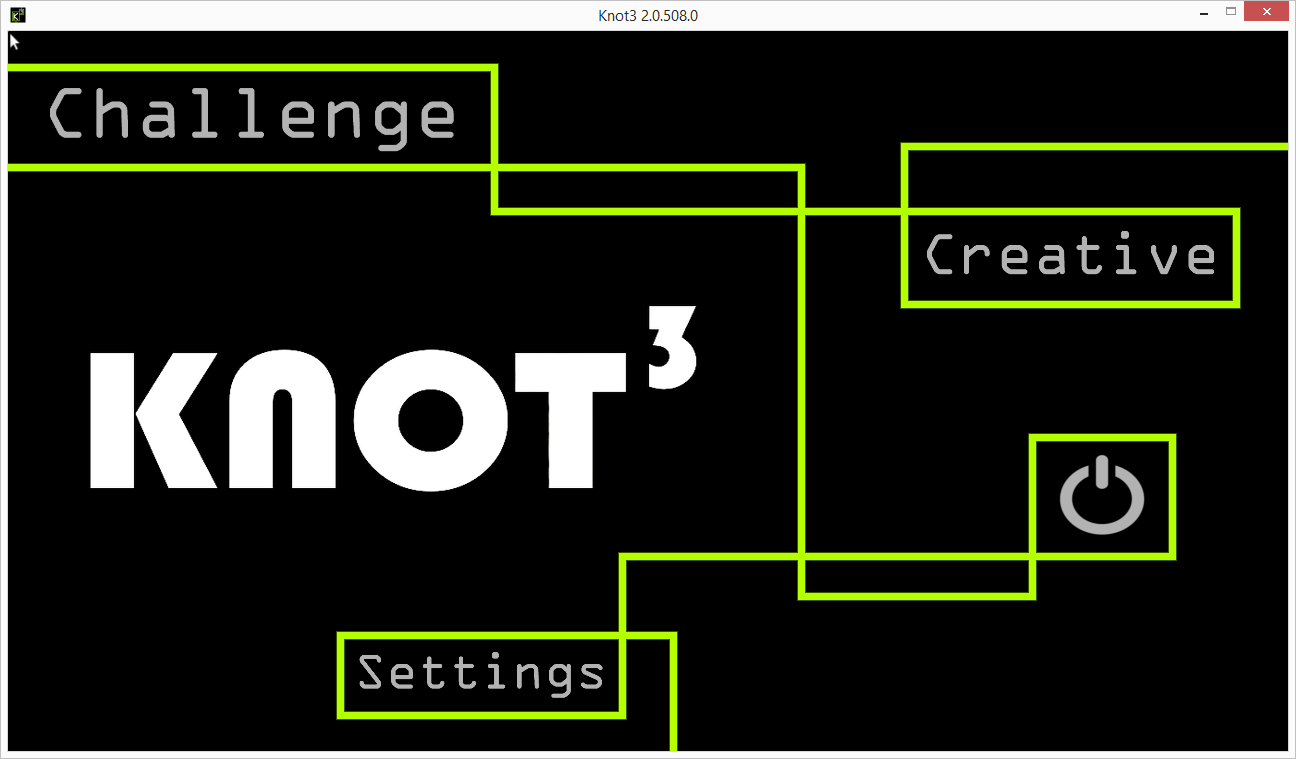
\includegraphics[width=\textwidth]{\ChangeMedia/Startmenue_(vorher).png}

	\end{figure}
	
~\\\mousecursor~\hyperref[Abschnitt:Aenderungen:Protokoll:Startmenue]{Siehe Startmenü-Änderung.} 



	% !TeX encoding = UTF-8
%



\section{Protokoll}
\label{Abschnitt:Aenderungen:Protokoll}













	% !TeX encoding = UTF-8
%



\subsection{Ge{"a}ndert}
\label{Abschnitt:Aenderungen:Protokoll:Behobene_Probleme}

Fehler die wir verbessert haben oder Ergänzungen werden hier beschrieben.\\




\subsubsection*{Credits}

% \subsubsection*{}








	% !TeX encoding = UTF-8
%



\newpage



\subsection{Nicht ge{"a}ndert}
\label{Abschnitt:Aenderungen:Protokoll:Nicht_behobene_Probleme}

Hier werden Probleme die wir nicht behoben haben oder nicht ändern konnten beschrieben.











	% !TeX encoding = UTF-8
%



\newpage



\subsection{Versch{"o}nerungen} % Juice it up!
\label{Abschnitt:Aenderungen:Protokoll:Verschoenerungen}













	
	% !TeX encoding = UTF-8
%



\chapter{Ausnahmen}
\label{Kapitel:Ausnahmen}

~\\











	% !TeX encoding = UTF-8
%



\section{Behandlung}
\label{Abschnitt:Ausnahmen:Behandlungen}

Probleme von denen wir Bescheid wissen werden so gehandhabt, dass die ungültige Aktion vom Spieler nicht durchführbar ist. Auch von uns unkontrollierbare Situationen, wie z.B.

\begin{itemize}

	\item Betriebssystem stellt keinen Dateispeicher mehr zur Verfügung.
	
	\item Speicherstand wird während des Spiels gelöscht.

\end{itemize}

oder unerwartete Fehler führen nie direkt zu einem Absturz.\\



	% !TeX encoding = UTF-8
%



\section{Meldungen}
\label{Abschnitt:Ausnahmen:Meldungen}













	
	% !TeX encoding = UTF-8
%



\chapter{Abschluss}
\label{Kapitel:Abschluss}

~\\



\section{Bewertung}
\label{Abschnitt:Abschluss:Bewertung}







	
	
	
	% Verzeichnisse
	%
	% \input{Inhalt/Verzeichnisse/Verzeichnisse}
	
	% Anhang
	%
	% !TeX encoding = UTF-8
%



\appendix



\chapter{Anhang}
\label{Anhang}













	% !TeX encoding = UTF-8
%



\section{Vollst{"a}ndige Fehlerliste}
\label{Anhang:Vollstaendige_Fehlerliste}













	% !TeX encoding = UTF-8
%



\section{Screenshots}
\label{Anhang:Aufnahmen}


~\\


\subsection*{Grafikfehler}



\newpage



\subsection*{Werkzeuge}


% Code-Coverage Report Build-Script

\begin{figure}[ht]

	\centering
	%\label{Abb:Werkzeuge:Code-Coverage_Build-Script}
	
	\includegraphics[width=\textwidth]{Inhalt/Anhang/Grafiken/Werkzeuge/Code-Coverage Report Build-Script.png}
	
	\caption{Build-Batch für die Erstellung des Testabdeckungs-Berichts.}

\end{figure}











\end{document}